%!TEX root = uw-ethesis.tex
% chktex-file 46 (ignore warnings about $...$)
% chktex-file 24 (ignore \label warning)

\chapter{Quadrotor Motion Planning}\label{chap:quad}

Quadrotors, as discussed in \autoref{chap:intro}, are growing in popularity for their many uses. Autonomous navigation for quadrotors is still in the early stages of development, although there are already some basic autonomous behaviours in use commercially; for example, many drones now support following a moving person to capture video footage. What makes quadrotor motion planning a truly interesting challenge is the fact that they occupy a 12D state space, and they are non-holonomic vehicles that are governed by nonlinear dynamics. The combination of high-dimensionality and nonlinearity render many current methods ineffective in the context of motion planning, for example the interval method~\cite{jaulin2001,Li2018}, which discretizes the state and control space with intervals, and suffers from the curse of dimensionality~\cite{Indyk1998}.

Before proceeding to the mathematics involved, it may be of interest to the reader to discuss our choice to use the term ``quadrotor''. But first, we begin by seeing that the word ``helicopter'' can be broken down into ``helico'', which is itself a combining form of ``helix'' (screw), and ``pter'' meaning ``wing''. Some people have referred to four-rotor helicopter UAVs as ``quadcopters'', but this terminology is ignorant of the Ancient Greek etymology of such words, as ``heli/copter'' is not the correct partitioning of the English word. So, the term ``quadrotor'' avoids the issue altogether, and its meaning is self-evident.

Now, in order to overcome the hurdles inherent in motion planning for such a complex system as a quadrotor, Ross Allen and Marco Pavone put forth a ``full-stack approach'' for real-time kinodynamic planning of such aerial vehicles~\cite{Allen2016}. First and foremost, a sampling-based planning approach was deemed necessary to deal with unknown environments online, and while SST* can handle the high-dimensionality and nonlinearity of the quadrotor system without needing a steering function, the incremental nature cripples its ability to plan effectively in an online setting. On the other hand, \gls{fmt}, with its pre-sampled states and its flexibility in allowing to perform much of the necessary pre-computation offline, is much more suited to online planning. For this reason, the authors centre their planning framework around a variant of FMT* called \texttt{kinoFMT}, introduced in \autoref{chap:prelims}. Once an approximate trajectory is found using this planning algorithm, trajectory smoothing is applied, and due the differentially flat nature of the quadrotor dynamics, it is then feasible to track the smooth trajectory with the proposed controller.

This chapter begins by analyzing the dynamical system that models quadrotor dynamics. Then, much of the work from~\cite{Allen2016} is described in various levels of detail, and conclusions are drawn from the efficacy of this approach. Finally, the main idea of using high-level temporal logic specifications using an abstracted Kripke structure, presented in \autoref{chap:sstpaper}, is applied to quadrotor kinodynamic planning \emph{with} steering under the aforementioned real-time planning framework.

\section{Quadrotor Model}

Before delving into the laws of motion for quadrotor systems, we begin by defining the underlying coordinate systems used in our analysis. In order to describe the position and velocity of the quadrotor, we need a fixed inertial reference frame (sometimes called the world frame) where Newton's laws hold. We will use the \gls{ned} configuration for this purpose with basis vectors $\{e_1, e_2, e_3 \}$. Along with the inertial frame, we define a body-fixed frame with basis $\{b_1, b_2, b_3\}$ whose origin coincides with the centre of mass of the quadrotor. The vectors $b_1$ and $b_2$ lie in the plane formed by the four rotors, and $b_3$ points in the direction opposite the applied thrust. See \autoref{fig:frames}.

\begin{figure}[h]
    \centering
    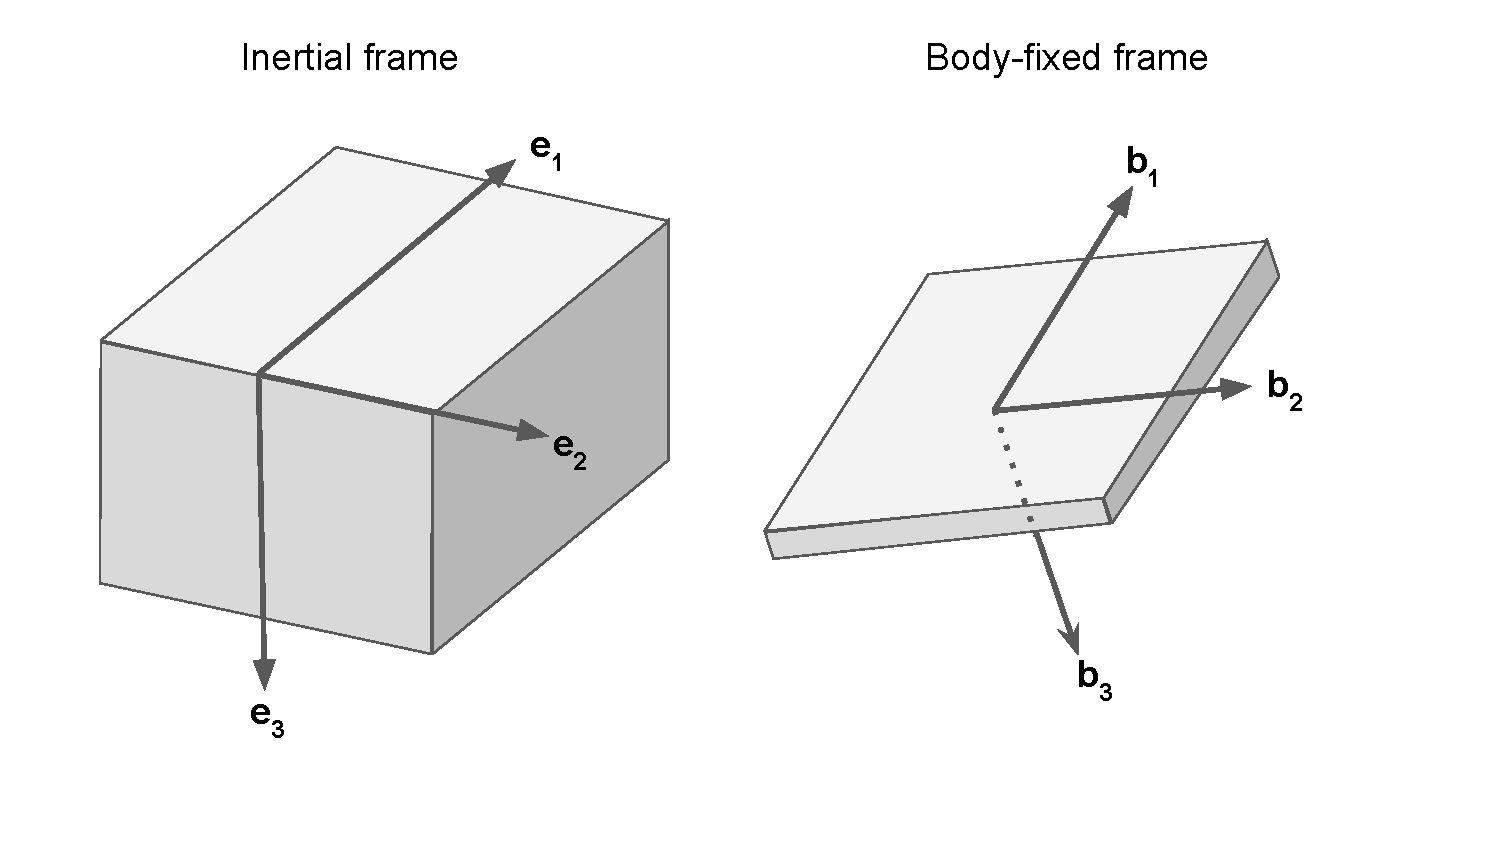
\includegraphics[scale=0.54]{./figures/frames}
    \caption[Inertial and body-fixed frames]{The inertial frame and the body-fixed frame are shown here, abiding by the NED convention.}
\label{fig:frames}
\end{figure}

Controlling a quadrotor involves adjusting the thrust applied to each of the four rotors. Note that opposite rotors rotate in the same direction, and adjacent rotors rotate in opposite directions; consequently, if all four rotors apply the same amount of thrust, the quadrotor will fly directly upward, and the angular momentum contributed by each rotor cancels so that there is zero rotational motion. Quadrotor motion is described in the space of all rigid body motions, namely the special Euclidean group $\text{SE}(3)$. This space has six degrees of freedom: translation in three dimensions, and rotation about each of the three body-fixed axes. However, given that there are only four control inputs, the quadrotor system is underactuated.

Rotational motion is often described by the Euler angles measuring yaw (about $b_3$), pitch (about $b_2$), and roll (about $b_1$). The use of Euler angles as state variables is not ideal, though, as singularities and jump-discontinuities arise as a result of restricting the domain of such angles. Recent work by Taeyoung Lee et al.\ instead takes a geometric control approach with a globally defined model to avoid such issues~\cite{Lee2010}, and we will make use of their work in modeling quadrotor dynamics. The important change they make is to replace the three Euler angle state variables with a single $3 \times 3$ matrix in the special orthogonal group, $\text{SO}(3)$, defined as follows:
\begin{equation}
    \text{SO}(3) = \{ R \in \R^{3 \times 3} \ \vert \ R^T R = I,\ \det(R) = 1 \}.
\end{equation}
The elements $R \in \text{SO}(3)$ are called rotation matrices, and they describe the current (or desired) attitude of the quadrotor. Given a vector $\vec{v}$ in the inertial frame,  



\section{Real-Time Motion Planning}\label{chap:quad:rtmp}

Blah.